\documentclass{article}
\usepackage{graphicx}
\usepackage{polski}
\usepackage[utf8]{inputenc}
\usepackage{graphicx}

\usepackage{subcaption}
\usepackage{algpseudocode}
\usepackage{amssymb}
\usepackage{listings}

\usepackage[a5paper]{geometry}
\graphicspath{ {./obrazki/} }
\begin{document}
\title{Model Chandrasekhara / Smoluchowskiego  - dowolna kombinacja pudeł}
\author{Piotr Piękos}

\maketitle

W tym dokumencie omówiony jest najogólniejszy przypadek modelu pudełek.
Zakładamy tutaj, że przejścia pomiędzy pudełkami tworzą łańcuch Markowa. Dodatkowo wierzchołki $x$ są opisane dwoma parametrami: \begin{itemize}
\item częstotliwością narodzin w danym wierzchołku $a_{xN}$
\item średnią długością przebywania w danym wierzchołku $a_{xS}$
\end{itemize}
W każdym wierzchołku mającym częstotliwość narodzin większą od zera cząstki regularnie sie "rodzą". W każdym wierzchołku po wejściu do niego (lub po narodzeniu w nim) losowana jest długość życia z rozkładu wykładniczego o zadanym dla wierzchołka parametrze. Po wyjściu cząstka przechodzi do następnego wierzchołka (lub umiera) zgodnie z macierzą przejść.

W dokumencie przedstawiony jest algorytm do symulacji, opis interfejsu oraz przykładowe ustawienia Łańcuchów wraz z trajektoriami.

\section{Interfejs}
Do opisu środowiska potrzebne są dwa pliki: \begin{itemize}
\item nodes - opisujący intensywność narodzin i długość życia we wierzchołku.
\item transitions - opisujący macierz przejść po wyjściu z wierzchołka
\end{itemize}

Format: \newline nodes jest to plik składający się z dwóch kolumn oddzielonych liczbami. Numer wiersza odpowiada numerowi wierzchołka (licząc od 1). Pierwsza kolumna to intensywność narodzin, druga to długość życia. \newline
transitions to surowy plik z macierzą przejść, kolumny oddzielone są spacjami. \textbf{ Pierwsza kolumna jest wyróżniona i oznacza przejście do wyróżnionego wierzchołka (śmierć)} 



Przykładowe środowiska są zawarte w folderach \begin{itemize}
\item kolko
\item koniczynka
\end{itemize}

\section{Opis algorytmu}

Wynikiem algorytmu będzie tabela ze zdarzeniami, gdzie zdarzeniem jest na przykład narodzenie cząsteczki, albo przejście jej z jednego pudła do innego. Oprócz informacji o zdarzeniu wiersz zawiera też czas wystąpienia zdarzenia

Algorytm składa się z dwóch części \begin{enumerate}
\item Narodziny cząsteczek
\item Podróżowanie
\end{enumerate}


W \textbf{pierwszej} części generujemy narodzone cząsteczki - wchodzimy do każdego "rodzącego" wierzchołka, symulujemy wszystkie narodziny które będą miały miejsce w danym wierzchołku podczas ustalonego horyzontu czasu.

W \textbf{drugiej} części "chodzimy" cząstkami między wierzcholkami. Ustalamy wierzchołek, dla wszystkich cząstek które aktualnie w nim przebywają losujemy czas życia oraz nowy wierzchołek. Nadpisujemy "obecny stan" i zapisujemy eventy do historii.

Taka realizacja algorytmu pozwala na wektorową realizację losowania czasów życia i przejść próbek co znacząco przyspiesza czas symulacji.




\section{Algorytm}
1. Narodziny cząsteczek
\begin{algorithmic}
\State for $x$ in rodzące wierzchołki:
\State \ \ \ \ Gen $N \sim \textit{Poiss}(a_{xN}t)$
\State \ \ \ \ for $i = 1$ to N do Gen $U_i \sim U(0, t)$
\State \ \ \ \ Dodaj pary ($x$, czas powstania) do historii oraz aktualnych wydarzeń
\end{algorithmic} 
"aktualne wydarzenia" oznaczają ostatnie wydarzenie z daną cząstką, jest ono nadpisywane i przechowuje informacje gdzie jest w danym "momencie" (nie jest to jednak robione chronologicznie z czasem)\newline
2. Podróżowanie
\begin{algorithmic}
\State w = 1, W - ilosc wierzchołków
\State while najmniejszy czas z aktualnych wydarzeń $< t$:
\State \ \ \ \ weź cząstki aktualnie będące w w.
\State \ \ \ \ Zasymuluj ich czas życia (z parametrem $a_{wN}$) oraz nowy wierzchołek
\State \ \ \ \ zaktualizuj aktualne wydarzenia i dodaj zmienione rzeczy do historii.
\State \ \ \ \ $w := w\ mod\  W + 1$ ($w \neq 0$, bo 0 to wierzchołek z martwymi cząsteczkami)
\State historia zawiera wszystkie wydarzenia, teraz wystarczy je posortować i odpowiednio przetransponować żeby mieć ilość cząsteczek w danej chwili
\end{algorithmic} 


\section{Przykłady}

\subsection{Przykładowe grafy}

Przykładami są 2 stworzone przeze mnie proste grafy demonstrujące główne funkcjonalności

Oznaczenia:

W wierzchołkach podane są intensywności rodzenia i parametry czasu życia w postaci $a_N | a_S$
na krawędziach podane są prawdopodobieństwa przejścia. Jeśli wychodzące krawędzie z wierzchołka nie sumują się do 1 to znaczy, że reszta to jest prawdopodobieństwo śmierci (wierzchołek w którym są martwe cząsteczki nie jest explicite rysowany)


\begin{figure}[h!]
\centering
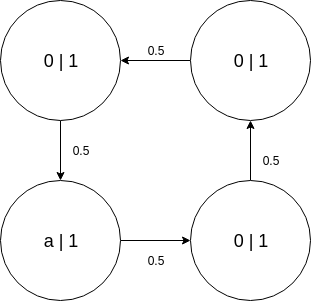
\includegraphics[width=0.6\linewidth]{kolko}
\caption{\textbf{Kolko}. W początkowym wierzchołku (lewym dolnym) cząstki rodzą się z intensywnością 1 oraz parametr rozkładu wykładniczego z którego losowany jest czas życia wynosi 1. W pozostałych wierzchołkach nigdy się nie rodzi żadna cząstka i parametr długości życia wynosi 1.}
\end{figure}

\begin{figure}[h!]
\centering
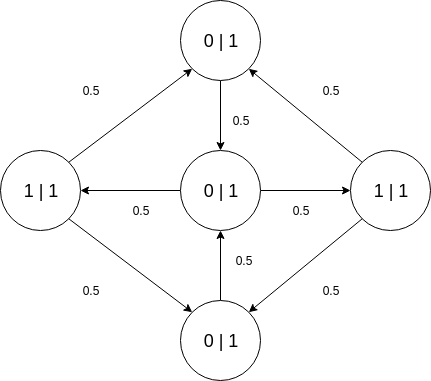
\includegraphics[width=0.6\linewidth]{koniczynka}
\caption{\textbf{Koniczynka}. Tutaj w dwóch (lewym i prawym) wierzchołkach rodzą się cząsteczki. Mogą umrzeć natomiast jedynie w górnym i dolnym.}
\end{figure}\newpage
Parametry wybrane jako 1 dla prostoty, oczywiście nic nie stoi na przeszkodzie, żeby były dowolne

\subsection{Kolko}
\subsection{Koniczynka}

\section{Uruchamianie symulacji}
\noindent kod do uruchamiania symulacji - w folderze wiecej\_pudla::
\begin{lstlisting}[language=bash]
  $ python3 sym.py t scheme_name output_file 
\end{lstlisting}
gdzie: \begin{itemize}
\item t - czas trwania symulacji
\item scheme\_name - nazwa schematu, folderu w którym są trzymane informacje o schemacie. Na przykład kolko albo koniczynka.
\item output\_file - nazwa pliku do którego ma się zapisać symulacja (csv)
\end{itemize}
\end{document}